The project you've been given is incomplete. In order for it to compile, you'll have to declare and attach a serial connexion to your pc.

The \textit{mbed} library provided by \mintinline{C}{"include "mbed.h"} defines the type \mintinline{C}{Serial} to declare a Serial connexion.

\begin{UPSTIactivite}[][Configure and connect the robot][][][To do]
 First, we need to declare and connect the serial port to communicate with the computer. Let's check the pin map to get the pin numbers we need to connect :
 \begin{center}
  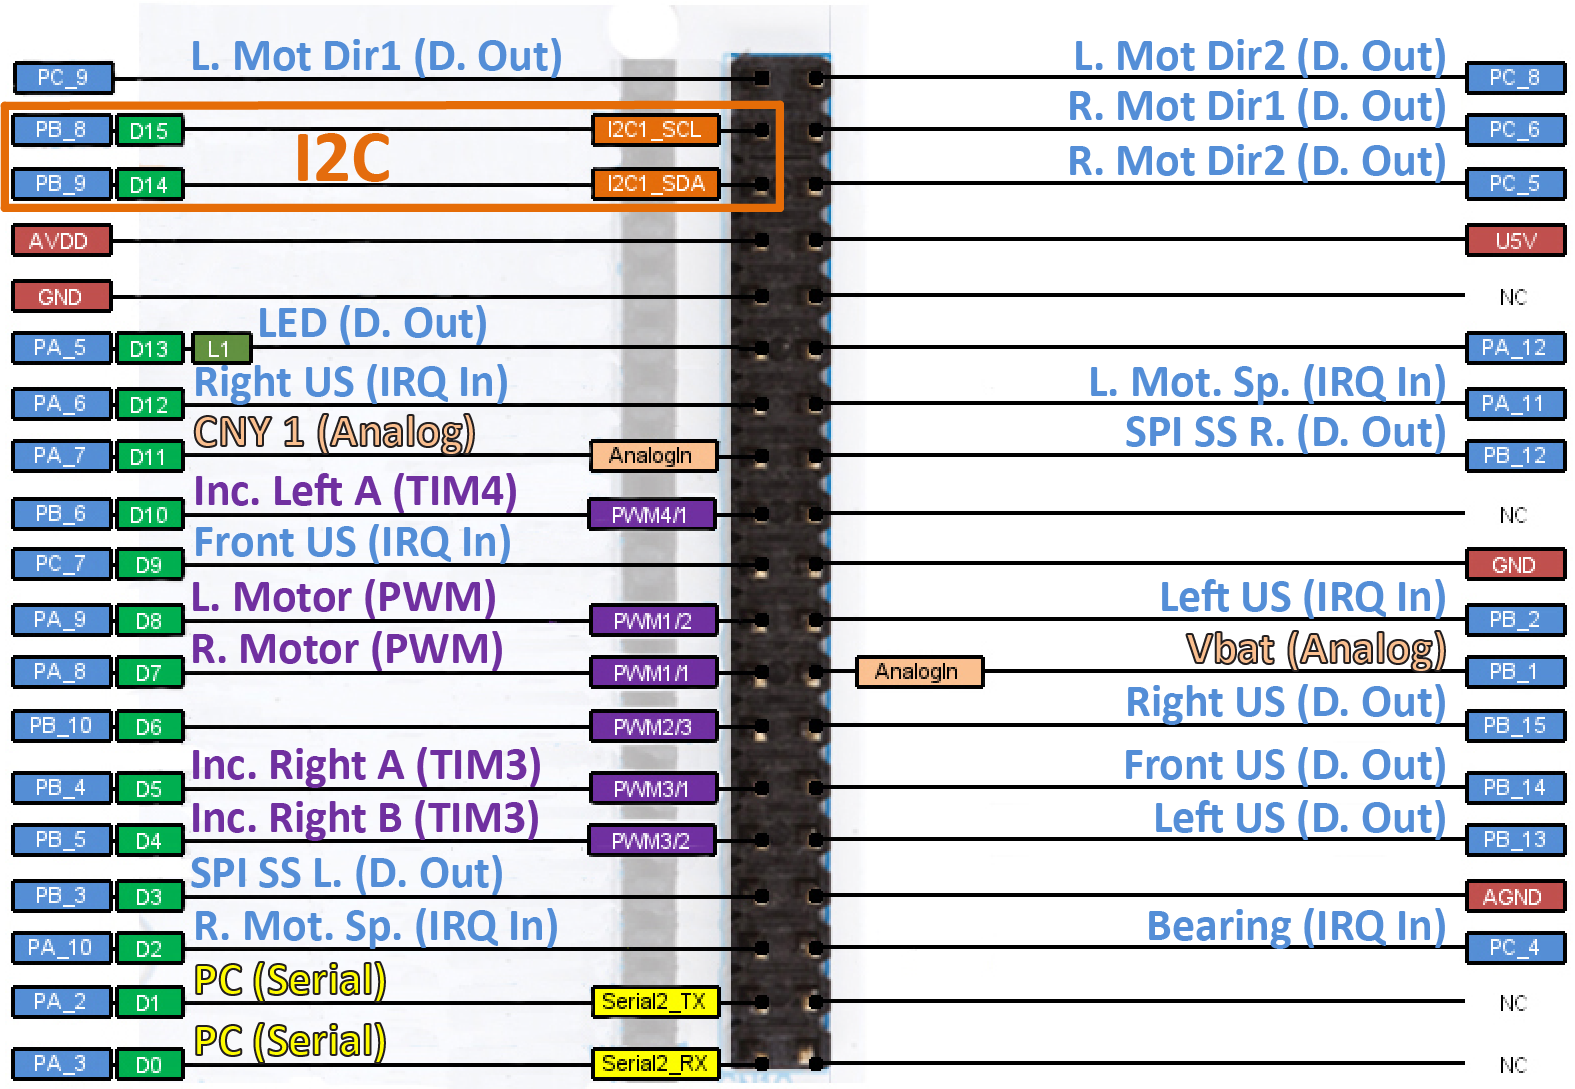
\includegraphics[viewport=0 0 190 30,height=6\fontcharht\font`\B,clip]{images/right_connectors}
 \end{center}
 \begin{enumerate}
  \item Open the file \mintinline{C}{includes/pin_connexions.h}
  \item Insert the following instruction \textbf{on line 25} in order to declare and connect the Serial port to Pins  \mintinline{C}{PA_2 and PA_3}. \mint{C}{Serial      pc      (PA_2, PA_3, 115200);}
  \item Click on the \textit{compile} button : 
\includegraphics[height=3\fontcharht\font`\B]{images/compile_button}
  \item Save the created executable on your computer.
  \item Connect the alimentation cables (red and black wires) to the robot and switch it on.
  \item Connect the USB cable to the computer and the NUCLEO card.
        \begin{itemize}
         \item The computer should detect the card and display it as a storage device.
        \end{itemize}
  \item Copy the executable to the card (drag and drop)
  \item Open a serial communication software on your computer
        \begin{enumerate}
         \item Open Teraterm software (You'll find it on your desktop)
         \item Choose Serial Connexion
         \item Change the port to STMicroelectronics Virtual Port and hit Ok
         \item In Setup -> Serial Port, change the baud rate to \num{115200}.
        \end{enumerate}
  \item Hit the RESET button (black) on the card
 \end{enumerate}
\end{UPSTIactivite}
